\documentclass{article}
\usepackage[margin=1in]{geometry}
\usepackage{amsmath,amsthm,amssymb}
\usepackage{bbm,enumerate,mathtools}
\usepackage{tikz,pgfplots}
\usepackage{chessboard}
\usepackage[hidelinks]{hyperref}
\usepackage{multicol} % Problem 35
\usepackage{xstring} % Difficulty command
\usetikzlibrary{shapes.geometric}

\newenvironment{question}{\begin{trivlist}\item[\textbf{Question.}]}{\end{trivlist}}
\newenvironment{note}{\begin{trivlist}\item[\textbf{Note.}]}{\end{trivlist}}
\newenvironment{references}{\begin{trivlist}\item[\textbf{References.}]}{\end{trivlist}}
\newenvironment{related}{\begin{trivlist}\item[\textbf{Related.}]\end{trivlist}\begin{enumerate}}{\end{enumerate}}

\newcommand\score[1]{
\pgfmathsetmacro\pgfxa{#1+1}
\tikzstyle{scorestars}=[
  star,
  star points=5,
  star point ratio=2.25,
  draw,
  inner sep=3pt,
  anchor=outer point 5
]
  \begin{tikzpicture}[baseline]
    \draw[opacity=0] (0,-0.5) rectangle (0,0.2); % Workaround for whitespace at the bottom.
    \foreach \i in {1,...,4} {
      \pgfmathparse{(\i<=#1?"yellow":"gray")}
      \edef\starcolor{\pgfmathresult}
      \draw (\i*4.5ex,0) node[name=star\i,scorestars,fill=\starcolor]  {};
    }
  \end{tikzpicture}
}

\newcommand{\difficulty}[1]{%
  \IfEqCase{#1}{%
      {1}{
        
\begin{tikzpicture}[scale=0.7, baseline=0.9mm]%
          \definecolor{slopegreen}{rgb}{0.0, 0.5, 0.0}%
          \fill[slopegreen] (0.5,0.5) circle (0.5);%
        \end{tikzpicture}%
      }%
      {2}{
        
\begin{tikzpicture}[scale=0.7, baseline=0.9mm]%
          \definecolor{slopeblue}{rgb}{0.0, 0.44, 1.00}
          \fill[slopeblue] (0,0) rectangle (1,1);%
        \end{tikzpicture}%
      }%
      {3}{
\begin{tikzpicture}[scale=0.7, baseline=0.9mm]\fill (0,0.5)--(0.5, 0)--(1,0.5)--(0.5,1)--cycle; \end{tikzpicture}}%
      {4}{
\begin{tikzpicture}[scale=0.7, baseline=0.9mm]\fill (0.25,0)--(0,0.5)--(0.25,1)--(0.5,0.5)--cycle; \fill (0.75,0)--(0.5,0.5)--(0.75,1)--(1,0.5)--cycle;\end{tikzpicture}}%
      % you can add more cases here as desired
  }[\PackageError{difficulty}{Undefined difficulty level: #1}{}]%
}%
\newcommand{\rating}[2]{\difficulty{#1}\\\score{#2}\\}

\begin{document}
\rating{2}{2}
We want to understand $k$-dimensional degree-$d$ B\'ezier curves with $d+1$ control points  $p_0, p_1, \dots, p_d$ in the set $\{0, 1, 2, \dots, n\}^k$: \[
  \vec{c}(t) = \sum_{i = 0}^d \binom{d}{i}t^i(1-t)^{d-i} p_i
\]
\begin{figure}[ht!]
  ~\hfill
  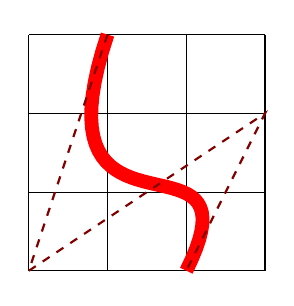
\begin{tikzpicture}
    \draw (0,0) grid (3,3);
    \draw [red, line width=5,  domain=0:1, samples=40]
      plot (
        {1*(1-\x)^3 + 0*3*\x^1*(1-\x)^2 + 3*3*\x^2*(1-\x)^1 + 2*\x^3},
        {3*(1-\x)^3 + 0*3*\x^1*(1-\x)^2 + 2*3*\x^2*(1-\x)^1 + 0*\x^3}
      );
    \draw[dashed, thick, red!50!black] (1,3)--(0,0)--(3,2)--(2,0);
  \end{tikzpicture}
  \hfill
  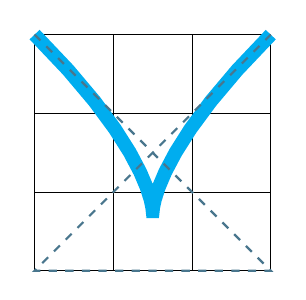
\begin{tikzpicture}
    \draw (0,0) grid (3,3);
    \draw [cyan, line width=5,  domain=0:1, samples=20]
      plot (
        {0*(1-\x)^3 + 3*3*\x^1*(1-\x)^2 + 0*3*\x^2*(1-\x)^1 + 3*\x^3},
        {3*(1-\x)^3 + 0*3*\x^1*(1-\x)^2 + 0*3*\x^2*(1-\x)^1 + 3*\x^3}
      );
    \draw[dashed, thick, cyan!50!black] (0,3)--(3,0)--(0,0)--(3,3);
  \end{tikzpicture}
  \hfill
  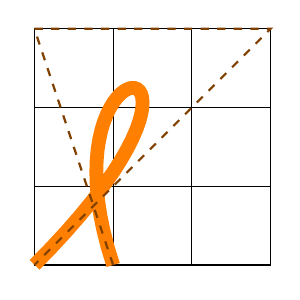
\begin{tikzpicture}
    \draw (0,0) grid (3,3);
    \draw [orange, line width=5,  domain=0:1, samples=40]
      plot (
        {1*(1-\x)^3 + 0*3*\x^1*(1-\x)^2 + 3*3*\x^2*(1-\x)^1 + 0*\x^3},
        {0*(1-\x)^3 + 3*3*\x^1*(1-\x)^2 + 3*3*\x^2*(1-\x)^1 + 0*\x^3}
      );
    \draw[dashed, thick, orange!50!black] (1,0)--(0,3)--(3,3)--(0,0);
  \end{tikzpicture}
  \hfill
  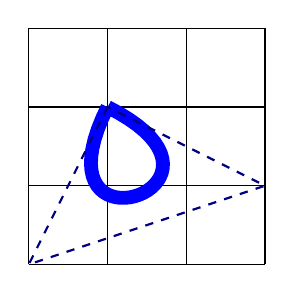
\begin{tikzpicture}
    \draw (0,0) grid (3,3);
    \draw [blue, line width=5,  domain=0:1, samples=40]
      plot (
        {1*(1-\x)^3 + 0*3*\x^1*(1-\x)^2 + 3*3*\x^2*(1-\x)^1 + 1*\x^3},
        {2*(1-\x)^3 + 0*3*\x^1*(1-\x)^2 + 1*3*\x^2*(1-\x)^1 + 2*\x^3}
      );
    \draw[dashed, thick, blue!50!black] (1,2)--(0,0)--(3,1)--(1,2);
  \end{tikzpicture}
  \hfill~
  \caption{
    Four examples of cubic B\'ezier curves with all four control points in $\{0,1,2,3\}^2$.
    The first has control points $(1,3)$, $(0,0)$, $(3,2)$, $(2,0)$.
    The second: $(0,3), (3,0), (0,0), (3,3)$.
    The third: $(1,0), (0,3), (3,3), (0,0)$.
    The fourth: $(1,2), (0,0), (3,1), (1,2)$.
  }
\end{figure}

\begin{question}
  For fixed $d$ the limit as $n \to \infty$, what is the probability of self-intersection?
\end{question}

\begin{related}
  \item How many distinct curves are there up to symmetry of the square.
  \item How many curves have a cusp?
  \item What can we say about the space of these curves when control points are instead in $[0,1]^k$? Is the set of non-self-intersecting curves connected in this setting?
  \item What are the extremal curves with respect to length, number of intersections, enclosed area, etc?
\end{related}
\begin{references}
  \item Wikipedia, ``\href{https://en.wikipedia.org/wiki/B%C3%A9zier_curve}{B\'ezier curve}.''
\end{references}

\end{document}
